\section{Schaltungsentwurf - Empfangseinheit}
Die Demodulation des Signals erfolgt im wesentlichen durch eine Tiefpass-Filterung. Das gesendete Signal muss allerdings erst vorbereitet werden. Dies geschieht durch eine Vorfilterung und anschließende Verstärkung. Ein Hochpass direkt am Ausgang der Empfangsdiode filtert DC-Anteile. Danach wird die Signalamplitude soweit verstärkt, dass der Signalverlauf wieder komplett rechteckig -dem ursprüglichen PWM-Signal entsprechend- verläuft. Dadurch wird die nachfolgende rekonstruierende Filterung durch den Butterwrorth-Tiefpass erst möglich.\\ Schlussendlich wird das zurückgewonnene Signal nach dem Rekonstruktionsfilter mit einer einstellbaren Endstufe final verstärkt, damit die Amplitude dem des gesendeten Signals entspricht.\\

%\begin{figure}[htbp]
%	\centering
%	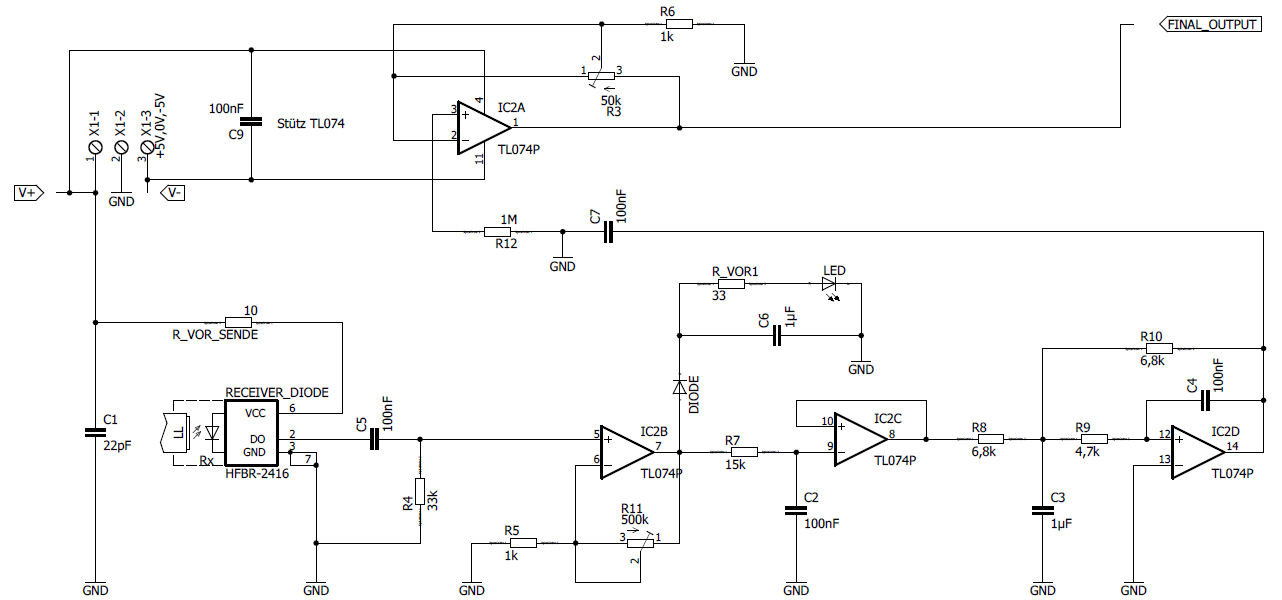
\includegraphics[angle=90, scale=0.36]{gfx/schaltung.png}
%	\caption{Empfängerschaltung (volles Querformat im Anhang)}
%\end{figure}